%%% Hlavní soubor. Zde se definují základní parametry a odkazuje se na ostatní části. %%%

%% Verze pro jednostranný tisk:
% Okraje: levý 40mm, pravý 25mm, horní a dolní 25mm
% (ale pozor, LaTeX si sám přidává 1in)
\documentclass[12pt,a4paper]{report}
\setlength\textwidth{145mm}
\setlength\textheight{247mm}
\setlength\oddsidemargin{15mm}
\setlength\evensidemargin{15mm}
\setlength\topmargin{0mm}
\setlength\headsep{0mm}
\setlength\headheight{0mm}
% \openright zařídí, aby následující text začínal na pravé straně knihy
\let\openright=\clearpage

%% Pokud tiskneme oboustranně:
% \documentclass[12pt,a4paper,twoside,openright]{report}
% \setlength\textwidth{145mm}
% \setlength\textheight{247mm}
% \setlength\oddsidemargin{15mm}
% \setlength\evensidemargin{0mm}
% \setlength\topmargin{0mm}
% \setlength\headsep{0mm}
% \setlength\headheight{0mm}
% \let\openright=\cleardoublepage

%% Použité kódování znaků: obvykle latin2, cp1250 nebo utf8:
\usepackage[utf8]{inputenc}

%% Ostatní balíčky
\usepackage{inconsolata}
\usepackage{paralist}
\usepackage{array}
\usepackage[shellescape]{gmp}
\usepackage{graphicx}
\usepackage{amsthm}
\usepackage{enumitem}
\usepackage[table]{xcolor}
\usepackage{tikz}
\usepackage{lmodern}
\usepackage{url}
\usepackage[T1]{fontenc}
\usepackage{listings}
\usepackage{pgfplots}
\usepackage{ifpdf}
\ifpdf
  \DeclareGraphicsRule{*}{mps}{*}{}
\fi

\bibliographystyle{plain}

\lstset {
	frame=bt,
    language=C++,
%    backgroundcolor=\color{black!5},
	backgroundcolor=\color{white},
%    numbers=left,
%    numbersep=5pt,
%	numberstyle=\tiny,
	xleftmargin=10pt,
	xrightmargin=10pt,
    basicstyle=\footnotesize\ttfamily,
    keywordstyle=\bfseries,
    aboveskip=15pt,
    belowskip=15pt,
    showstringspaces=false
}

%% Balíček hyperref, kterým jdou vyrábět klikací odkazy v PDF,
%% ale hlavně ho používáme k uložení metadat do PDF (včetně obsahu).
%% POZOR, nezapomeňte vyplnit jméno práce a autora.
\usepackage[unicode]{hyperref}   % Musí být za všemi ostatními balíčky
\hypersetup{pdftitle=Bobox Runtime Optimization}
\hypersetup{pdfauthor=Lukáš Krížik}
\hypersetup{pdfborder={0 0 0}}

\usepackage{epstopdf}

\usetikzlibrary{arrows,fit,positioning,calc,patterns,shapes.multipart,backgrounds} 
\tikzset{
    %Define standard arrow tip
    >=stealth',
    %Define style for boxes
    title/.style={
           text centered},
    % Define arrow style
    pil/.style={
           ->,
           thick,
           shorten <=3pt,
           shorten >=3pt,}
}

%%% Drobné úpravy stylu

% makro for code text definition
\def\code#1{\texttt{#1}}

% Tato makra přesvědčují mírně ošklivým trikem LaTeX, aby hlavičky kapitol
% sázel příčetněji a nevynechával nad nimi spoustu místa. Směle ignorujte.
\makeatletter
\def\@makechapterhead#1{
  {\parindent \z@ \raggedright \normalfont
   \Huge\bfseries \thechapter. #1
   \par\nobreak
   \vskip 20\p@
}}
\def\@makeschapterhead#1{
  {\parindent \z@ \raggedright \normalfont
   \Huge\bfseries #1
   \par\nobreak
   \vskip 20\p@
}}
\makeatother

% Toto makro definuje kapitolu, která není očíslovaná, ale je uvedena v obsahu.
\def\chapwithtoc#1{
\chapter*{#1}
\addcontentsline{toc}{chapter}{#1}
}

\begin{document}

% Trochu volnější nastavení dělení slov, než je default.
\lefthyphenmin=2
\righthyphenmin=2

%%% Titulní strana práce

\pagestyle{empty}
\begin{center}

\large

Charles University in Prague

\medskip

Faculty of Mathematics and Physics

\vfill

{\bf\Large MASTER THESIS}

\vfill

\centerline{\mbox{\includegraphics[width=60mm]{../img/logo.eps}}}

\vfill
\vspace{5mm}

{\LARGE Lukáš Krížik}

\vspace{15mm}

% Název práce přesně podle zadání
{\LARGE\bfseries Bobox Runtime Optimization}

\vfill

% Název katedry nebo ústavu, kde byla práce oficiálně zadána
% (dle Organizační struktury MFF UK)
The Department of Software Engineering

\vfill

\begin{tabular}{rl}

Supervisor of the master thesis: & RNDr. Filip Zavoral, Ph.D. \\
\noalign{\vspace{2mm}}
Study programme: & Informatics \\
\noalign{\vspace{2mm}}
Specialization: & Software Systems \\
\end{tabular}

\vfill

% Zde doplňte rok
Prague 2014

\end{center}

\newpage

%%% Následuje vevázaný list -- kopie podepsaného "Zadání diplomové práce".
%%% Toto zadání NENÍ součástí elektronické verze práce, nescanovat.

%%% Na tomto místě mohou být napsána případná poděkování (vedoucímu práce,
%%% konzultantovi, tomu, kdo zapůjčil software, literaturu apod.)

\openright

\noindent
Dedication.

\newpage

%%% Strana s čestným prohlášením k diplomové práci

\vglue 0pt plus 1fill

\noindent
I declare that I carried out this master thesis independently, and only with the cited
sources, literature and other professional sources.

\medskip\noindent
I understand that my work relates to the rights and obligations under the Act No.
121/2000 Coll., the Copyright Act, as amended, in particular the fact that the Charles
University in Prague has the right to conclude a license agreement on the use of this
work as a school work pursuant to Section 60 paragraph 1 of the Copyright Act.

\vspace{10mm}

\hbox{\hbox to 0.5\hsize{%
In ........ date ............
\hss}\hbox to 0.5\hsize{%
signature of the author
\hss}}

\vspace{20mm}
\newpage

%%% Povinná informační strana diplomové práce

\vbox to 0.5\vsize{
\setlength\parindent{0mm}
\setlength\parskip{5mm}

Název práce:
Bobox Runtime Optimization
% přesně dle zadání

Autor:
Lukáš Krížik

Katedra:  % Případně Ústav:
Katedra softwarového inženýrství
% dle Organizační struktury MFF UK

Vedoucí diplomové práce:
RNDr. Filip Zavoral, Ph.D.
% dle Organizační struktury MFF UK, případně plný název pracoviště mimo MFF UK

Abstrakt:
Cílem této diplomové práce je vytvořit nástroj na optimalizaci kódu pro paralelní prostředí Bobox. Nástroj redukuje počet krátce a dlouze běžících úloh na základě statické analýzy kódu. Některé případy krátce běžících úloh způsobují zbytečné přeplánování. Pokud plánovač nemá dostatek informací o dané úloze, plánovač může úlohu naplánovat, i když tato úloha nemá všechny potřebné vstupní data. Pro odstranění krátce běžící úlohy, nástroj analyzuje použití vstupních dat a informuje plánovač. Dlouze běžící úlohy můžou v některých případech potlačit paralelismus. Větší granularita úloh může znatelně vylepšit časy běhu v paralelním prostředí. Pro odstranění dlouze běžících úloh, nástroj musí byt schopen vyhodnotit složitost kódu a vložit příkaz pro přeplánování na vhodné místo.
% abstrakt v rozsahu 80-200 slov; nejedná se však o opis zadání diplomové práce

Klíčová slova:
bobox, statická analýza kódu, optimalizace, složitost kódu, clang
% 3 až 5 klíčových slov

\vss}\nobreak\vbox to 0.49\vsize{
\setlength\parindent{0mm}
\setlength\parskip{5mm}

Title:
Bobox Runtime Optimization
% přesný překlad názvu práce v angličtině

Author:
Lukáš Krížik

Department:
The Department of Software Engineering
% dle Organizační struktury MFF UK v angličtině

Supervisor:
RNDr. Filip Zavoral, Ph.D.
% dle Organizační struktury MFF UK, případně plný název pracoviště
% mimo MFF UK v angličtině

Abstract:
The goal of this thesis is to create a tool for an optimization of code for the task-based parallel framework called Bobox. The optimizer tool reduces a number of short and long running tasks based on a static code analysis. Some cases of short-running tasks cause an unnecessary scheduling overhead. The Bobox scheduler can schedule a task even though the task does not have all input data. Unless, the scheduler has enough information not to schedule such task. In order to remove such short-running task, the tool analyses its input usage and informs the scheduler. Long-running tasks inhibit a parallel execution in some cases. A bigger task granularity can significantly improve execution times in a parallel environment. In order to remove a long-running task, the tool has to be able to evaluate a runtime code complexity and yield a task execution in the appropriate place.
% abstrakt v rozsahu 80-200 slov v angličtině; nejedná se však o překlad
% zadání diplomové práce

Keywords:
bobox, static code analysis, optimization, code complexity, clang
% 3 až 5 klíčových slov v angličtině

\vss}

\newpage

%%% Strana s automaticky generovaným obsahem diplomové práce. U matematických
%%% prací je přípustné, aby seznam tabulek a zkratek, existují-li, byl umístěn
%%% na začátku práce, místo na jejím konci.

\openright
\pagestyle{plain}
\setcounter{page}{1}
\tableofcontents

%%% Jednotlivé kapitoly práce jsou pro přehlednost uloženy v samostatných souborech
\chapter{Introduction}
The Bobox project is a task-based framework for parallel computing. In such a framework, short-running tasks cause bigger CPU consumption by the framework itself and long-running tasks can inhibit the parallel execution. A static code analysis can be used to detect and eliminate such execution paths in the user code. Since the core and interface language of the Bobox framework is C++, static code analysis becomes more difficult in proportion to the lack of tools. This has been the biggest pitfall for any static analysis of C++ code. However, it has become less marginal with a growing support for tooling in the Clang compiler front-end~\cite{clang}. Clang exposes C++ code as a user-friendly \emph{Abstract Syntax Tree (AST)}~\cite{ast} structure.

\section{Goals}
Apart from this text, the main asset of this thesis is a tool for optimizing code using the Bobox framework. By analysing AST, the tool is able to diagnose and potentially transform user code to eliminate both short and long execution paths. There is an implementation of the two different patterns of unoptimized usage in the context of this thesis. However, the tool is designed to be easily extensible with new optimization methods. Both implemented optimization methods are able to inject new code to give the Bobox internal facilities information about the user code structure. The tool is implemented using the Clang tooling interface~\cite{clang-documentation}. Therefore, it inherits all the Clang limitations, such as its platform support.

\section{Structure of the thesis}
The second chapter begins with a brief description of the Bobox framework, in order to familiarize a reader with its underlying mechanisms. The reader should understand why the user code can be optimized using the transformations mentioned later in chapters related to specific optimization methods.

The third chapter describes the problems of static code analysis first of all in general, and then specifically for the C++ language since it is the core and interface language of the Bobox framework. The chapter also describes the possible approaches to a static code analysis of C++ code, their advantages and disadvantages, the internal implementation, and the user interface and limitations. The last section in this chapter addresses related work.

Because the chosen approach to implement the optimizer tool was the Clang tooling interface, Chapter~\ref{chapter-clang} is dedicated to its detailed description. Tools implemented on top of the Clang front-end are equipped with an abstract syntax tree representation of code. One section describes the design of this data structure, and the possibilities of its traversal. Possibilities of source-to-source transformations are described in the following section. The Clang front-end itself provides multiple interfaces for an implementation of static code analysis tools.

The next two chapters introduce implemented optimization methods. Each chapter contains sections with information related to the Bobox framework, a detailed description of the algorithms used to detect an unoptimized usage of the framework and other details of the implementation.

Chapter~\ref{chapter-design} offers a high-level look at the tool design and some details of optimizer implementation. The following chapter contains achieved results of the described scenarios. The last chapter discusses conclusions and the future work.
\chapter{Bobox}
Nowadays, increasing performance comes with an increasing number of computational units due the attainment of the physical limits of current technologies. Parallel programming becomes more and more important in the development of performance expensive software to use all the silicon hardware provides. The thread-based approach to achieve parallelism creates a lot of complexity for a programmer to maintain, and it is also not well scalable. It becomes important to abstract the underlying parallel environment to a programmer. The Bobox framework~\cite{bobox-4, bobox} addresses this issue by providing an interface for task-based parallel programming. Such an approach relieves the programmer of handling thread-based programming problems such as synchronization, most technical details (e.g., cache hierarchy, CPU architecture) and communication. Apart from that, task-based programming also allows for better hardware utilization.

According to Bednárek et al.~\cite{bobox-1}, the Bobox framework is \textit{"more useful for data processing scenarios, like database query evaluation or stream processing"}. Without further details, under the hood, the framework has been equipped with a fixed number of worker threads, each one with an own scheduler, and two task queues for every computational unit for a better utilization of CPU caches, using the task stealing mechanism. Communication between tasks uses a column-based data model, the most significant implementation detail that favours data processing problems. Each task has zero or more inputs and zero or more outputs. A single output can be connected to zero or more inputs. A task is scheduled to be executed when it has an unprocessed input.

The Bobox framework provides a C++ library as the interface to its runtime environment. Task granularity is represented by classes derived from the Bobox base class for a task. This base class is called a \emph{box}.

\section{Design and terminology}
\label{bobox-terminology}
The runtime environment handles the implementation details of the task-based parallel environment such as scheduling and the parallel execution of tasks, data transport and control flow. A programmer uses a declarative way to provide the environment with a \emph{model} which defines the way individual tasks are interconnected. The model is used to create a \emph{model instance} which is the base for creating a \emph{user request}. The user request contains only very little additional information compared to the model instance.

After a programmer provides the environment with a user request, he no longer has control over its execution. The framework provides only information about whether it has finished executing the request. The provided user request is divided into individual tasks. When a task is ready to be executed, it is added to the task pool. A worker thread then retrieves the task from the task pool and invokes it.

The basic element of model instance is an element representing a task, called a box. In every model instance, there is a special box called an \emph{initialization box}. This box is responsible for the creation of the initialization input data of all the other boxes in the model. The framework executes this task at the beginning of a request evaluation, and its only goal is to send data to its only output.

Data is sent using an \emph{envelope}, a column-based data structure. An empty envelope is a special type of envelope called a \emph{poisoned pill}. When a box receives a poisoned pill in its input, there will be no more data sent to this input. All the paths of model instances are required to end in another special type of box called a \emph{termination box}. When this box receives a poisoned pill, the execution is finished and the pipeline is deallocated.

\section{Boxes}
\label{bobox-boxes}
Boxes, as the representation of Bobox framework tasks, are executed in three steps.

\begin{enumerate}
\item The first step is the \emph{prologue}, when the box creates a snapshot of its inputs and stores this snapshot in member variables so the user code can access it. The prologue communicates with the runtime environment, and synchronization is needed.
\item The second step called \emph{action} is the main place for a user code execution. User code can communicate with the runtime environment using only specific member functions, e.g., it can send an envelope to its output. This approach creates a transparent parallel environment for programmers, relieving them of issues related to the parallel execution.
\item The last step is the \emph{epilogue}. The step handles the scheduling of the next task based on two criteria. A task is scheduled again,

\begin{enumerate}
\item if it has got an unprocessed input and it has processed some input in the action step.
\item if it requested to be scheduled again.
\end{enumerate}

There is a reason why box is not scheduled again if it has got unprocessed input and it has not processed any input during the execution. It will most likely wait for another input, e.g., the join operation in a database when a task is not executed until it has received data from both inputs. The option to explicitly request another scheduling is there for cases when a single box creates a large output. A task should not run for a long period of time. It can create a large output, and thus congest internal buffers used for communication. A task running for a long time on a single worker thread can also create a bottleneck for a parallel execution when many other tasks wait for the input from this task.

\end{enumerate}

Boxes are main objects of the interest for optimization, because they are the main location for the user code. Based on the static analysis of the action step, additional code can be injected to provide Bobox internal facilities with information about the task.

\section{Usage}
\label{bobox-usage}
To implement a Bobox task, a programmer has to inherit from the \code{basic\_box} base class. The action step is represented by one of the virtual member functions from Listing~\ref{bobox-action-step}. A programmer is expected to override one of them. The synchronous version is called when all prefetched envelopes are available. The asynchronous version is called when the envelope on the input which is being \textit{listened} is available.

\begin{lstlisting}[caption={The code representations of the box action step.},label={bobox-action-step}]
virtual void sync_body();
virtual bool async_body(inarc_index_type inarc);
\end{lstlisting}

A programmer can also associate names to particular inputs and outputs using helper macros from the Bobox library, see Listing~\ref{bobox-macros}. The code is easier to comprehend and maintain when box inputs or outputs are referred to by names instead of using indexes.

\begin{lstlisting}[caption={The helper macros for mapping of names to inputs and outputs.},label={bobox-macros}]
#define BOBOX_BOX_INPUTS_LIST(...)
#define BOBOX_BOX_OUTPUTS_LIST(...)
\end{lstlisting}

The implementation of a task is straightforward for a C++ programmer using only C++ core language features. Unfortunately, C++ syntax is not convenient for expressing a definition of the whole execution model. The language developed to such purpose is called \emph{Bobolang}~\cite{bobolang}. Listing~\ref{bobox-bobolang} shows an example of a model definition in the Bobolang language.

\begin{lstlisting}[caption={An example of the Bobolang usage.}, label={bobox-bobolang}]
model main<()><()> {
    bobox::broadcast<()><(),()> broadcast;
    Source<()><(int)> source1(odd=true), source2(odd=false);
    Merge <(int),(int)><(int)> merge;
    Sink <(int)><()> sink;
	
    input -> broadcast;
    broadcast[0] -> source1;
    broadcast[1] -> source2;
    source1 -> [left]merge;
    source2 -> [right]merge;
    merge -> sink -> output;
}
\end{lstlisting}

\section{Cooperative scheduling}
Due to the character of the framework scheduler, the user code directly affects the scheduling of tasks and thus the overall performance of an execution. The framework provides ways of manipulating the task scheduling. For example, a task can give up its execution before it finishes naturally. A task can also inform the scheduler that it should not be executed before all the input data is available. Based on the static code analysis of the user code, the optimizer tool can inject function calls into the user code to affect framework scheduling.
\chapter{Static code analysis}
Detection of errors in code early in development process is important for reducing development cost. The most commonly used process to detect errors as soon as possible is called \emph{code review}. Static code analysis can be considered to be automated code review.

One of the biggest pitfalls of code review is high price if big portion of development budget consists of developer salaries. Two or more people read code looking for a way to improve it, finding and fixing errors or potential errors that can become real errors in future, or performance issues. Quality of code review decreases with time spent reading code. Developers need to rest to increase quality of their code review.

Compiler warnings can be considered to be very basic static code analysis performed by compiler. It warns programmer about suspicious parts of code it detected in compilation process. It is good practice to turn on all compiler warnings and compile code without any detected. The most commonly used compilers provide switch to consider warnings as an errors. Software development companies often create rules to force programmers to produce warning-less code, or simply using mentioned compiler switch in development environment to implicitly remove compilation warnings.

There is not much compilers can do in diagnosing more complex errors. It is not their primary goal which is code compilation and more advanced diagnostic could increase compilation times. In context of this thesis, where C++  is the analysed language, compilation times do really matter. Furthermore, there is no need to produce any binary when analysing code. Developers of tool for static code analysis would like to step in right after semantic analysis finished when there is enough understanding of source code. It is up to programmer whether he reuses front-end of compiler or implements his own.

\section{Pitfalls}
Due to complexity of C++ core language, there are only a very few fully C++ compliant, open-source and freeware\footnote{Proprietary compilers could do the job as well, but freeware compilers are preferred ones.} compilers. The two most known are \emph{GCC, the GNU Compiler Collection}, and \emph{Clang/LLVM}. Apart from standard syntax for procedural programming, C++ standard includes Turing-complete template metaprogramming language. Simplified, compiler needs to \textit{execute} code in order to generate code that is eventually compiled into native code. As an example of language complexity, implementation of \emph{export} feature, which allows programmers to define template code in one translation unit and use in different, was so huge task for compiler vendors\footnote{Only one compiler vendor was able to implement it, \emph{Comeau C/C++}.} that this feature was eventually removed from language\footnote{Keyword has remained in language for future purpose.}. Based on given facts, it would be extremely difficult and unwise to individually implement own C++ front-end.

This chapter will cover some of the possible approaches for creating static code analysis tool apart from using Clang which is covered by the next chapter.

\section{GCC - the GNU Compiler Collection}
GCC is compiler with 26 years old great history and is well established in C++ software development world. Many helper tools for build environment support GCC in some way, and yet programmers were struggling with writing static code analysis tools for C++. Why was not GCC used? Cite from \emph{Sparse FAQ} \cite{sparse} partially covers the answer.\\

\textit{"Gcc is big, complex, and the gcc maintainers are not interested in other uses of the gcc front-end.  In fact, gcc has explicitly resisted splitting up the front and back ends and having some common intermediate language because of religious license issues - you can have multiple front ends and back ends, but they all have to be part of gcc and licensed under the GPL."}\\

The first sentence, especially the first few words, is the main reason programmers have not started using GCC front-end to create tools for static code analysis.

\begin{itemize}
\item It is very hard to learn for beginners.

\item Even though GCC consists of front-end, middle-end and back-end, it \textit{feels} monolithic by design. It is very difficult to decouple front and back ends.

\item GENERIC and GIMPLE\footnote{Those are names for different representations of AST. GIMPLE is subset of GENERIC for code optimizations.} representations of code are not intuitive.

\item GCC does not keep track of tokens locations in source code, e.g., it does not keep track of macro expansions. Therefore, it is very difficult to refactor code correctly.

\item Code is optimized when it is parsed so AST does not correspond to source code, e.g., \code{x-x} is optimized to be \code{0}. It is extremely difficult to refactor code based on such optimized AST.
\end{itemize}

One disadvantage that can be argued, but it is disadvantage for me personally.

\begin{itemize}
\item Code base is written mainly in C language. Even though there is ongoing transition to C++, it is not going to change design of the compiler. Transition will introduce only a very few and simple C++ features, e.g., STL containers such as \code{std::vector}, smart pointers to partially replace GCC internal garbage collection or templates.
\end{itemize}

\section{Elsa: The Elkhound-based C/C++ Parser}
Even a smaller group of developers is able to create relatively nice C++ compiler front-end. Elsa is such an example. It provides programmer with user-friendly AST representation of code, which is designed in the way it is easily extensible without writing single line of C++ code. For AST traversal, front-end provides mechanism designed as \emph{Visitor pattern}. The other way is to traverse tree manually by following edges. Visitor pattern is useful for context insensitive traversal. Within chapter dedicated to Clang, reader will discover that both approaches are very similar to what Clang provides to developer.

The biggest disadvantage of Elsa is that its development stopped long time ago in 2005 when different project, called \emph{Oink}, which uses Elsa front-end, started. Then Oink development stopped before year 2011 when C++ experienced its \textit{renaissance} with the new approved standard since year 2003 which introduced big changes to core language and library. Therefore, there is almost no support for new C++11 language features. Oink as well as Elsa does not have integrated preprocessor and so it is extremely difficult to map AST with locations in source code. Elsa also suffers from lower speed, but it can be negligible disadvantage for smaller projects.

\section{VivaCore/OpenC++}
Library was created as basis for \emph{PVS-Studio} static code analyser for C/C++ code. VivaCore is derived from older \emph{OpenC++ (OpenCxx)} library. The idea of using OpenC++ appeared when team was implementing \emph{Viva64} library. They were making many changes to OpenC++ and because lack of resources they did not continue to improve it\footnote{Many changes did not fit into OpenC++ ideology so they would need to adapt and allocate new resources for such process.}, but rather developed their own library. Library has become popular and has been used as basis by other very popular tools such as  \emph{VisualAssist} by \emph{Whole Tomato Software}, \emph{Doxygen}, \emph{Gimpel Software PC-Lint}, \emph{Parasoft C++test} and more.

\begin{figure}[t!]
\label{vivacore}
\caption{Design of VivaCore library.}
\centering
\vspace{0.5cm}
\begin{tikzpicture}[node distance=1.25cm, every text node part/.style={align=center}]
 \node(preprocessor) {External \\ preprocessor};
 \node(internal) [below=of preprocessor] {Preprocessor \\ subsystem};
 \node[below=of internal](lexer) {Lexer};
 \node[below=of lexer](parser) {Parser};
 \node[below=of parser](walker) {PT Walker};
 \node[below=of walker](metaprogram) {Metaprogram \\ subsystem};
 
 \path[<->] (preprocessor) edge node {} (internal);
 
 \path[*-*] (internal) edge node {} (lexer)
 	        (lexer) edge node {} (parser)
 	        (parser) edge node {} (walker)
 	        (walker) edge node {} (metaprogram);
 	        
 \node(utility) at (-5, -6.25) { C/C++ \\ Analysis \\ Library and \\ Utilities };
 
 \path[dashed] (utility) edge node {} (internal)
               (utility) edge node {} (lexer)
               (utility) edge node {} (parser)
               (utility) edge node {} (walker)
               (utility) edge node {} (metaprogram);
 
 \node(viva) at (-2.5, -11.5) {\LARGE\textbf{VivaCore}};
 
 \node[above=of internal, yshift=-1.25cm] (dummyfit){};
 
 \begin{pgfonlayer}{background}
  \node [draw,fit=(internal) (lexer) (parser) (walker) (metaprogram) (viva) (utility) (dummyfit)] {};
 \end{pgfonlayer}
 
\end{tikzpicture}
\end{figure}

The first step of code analysis is to use preprocessor. Library uses external preprocessor what becomes its biggest disadvantage in source-to-source transformation process. Without integrated preprocessor, it is next to impossible to track macro expansion and actual location of symbols in source code.

Preprocessed input is then passed to library. Two library subsystems process code before it gets to lexical analysis. Input subsystem responsible for putting preprocessed code into internal data structures is the first. The second step is internally called \emph{Preprocessor}, but it does not preprocess input in the meaning of C++ preprocessor. It is responsible for two operations:

\begin{itemize}
\item Splitting code into strings and dividing them into two logical groups. One is for system libraries and the second one is for user code. Library user can choose whether he wants to analyse system code or just user code.
\item Removing C++ non-related strings specific for compiler, e.g., \code{SA\_Success} and \code{SA\_FormatString} can be found in Visual Studio headers.
\end{itemize}

Next step is lexical analysis. Output of \emph{Lexer} can be used for basic metrics or syntax highlighting. VivaCore allows easy modifying set of tokens for lexical analysis.

VivaCore provides user with \emph{parse tree (PT)} called also \emph{derivation tree (DT)} as an output of syntactic analysis. Parse tree differs from abstract syntax tree in the way it contains nodes representing derivation rules used in syntactic analysis. The word \emph{abstract} comes from the reasoning that structure hides the way it was constructed. It is actually possible to traverse PT as it was AST. VivaCore`s PT defines two basic sets of nodes with ancestors in \code{NonLeaf} and \code{Leaf} base classes which have \code{PTree}\footnote{\code{PTree} has \code{LightObject} as its base class used in GC.} class as their common ancestor declaring the only pure virtual member function:

\begin{lstlisting}[caption={Pure virtual member function of base for VivaCore parse tree node.}]
virtual bool IsLeaf() const = 0;
\end{lstlisting}

It is the only function necessary to be overridden in inherited classes letting their design more flexible.

Probably the most interesting part of library interface is tree traversal. There are three different \emph{walker} classes implemented for this purpose.

\begin{description}
\item[Walker] is responsible for walking over basic C++ constructions.
\item[ClassWalker] handles C++ class specific features.
\item[ClassBodyWalker] traverses body of C++ class.
\end{description}

It is possible to traverse PT multiple times so user can traverse code for measurements at first and later, in further traversals, he may modify PT. If user modifies tree nodes, it may occur that tree is rebuilt.

\section{Related work}
Code quality in a huge projects is hard to maintain using only code review since there are many code related commits every day (e.g. Crysis 2 multiplayer had $\sim$100-150 code related commits every day collecting 130 different developers over the last year of development \cite{crysis}.) and providing people resources for code review would be inefficient. Instead of that, companies use tools for static code analysis and diagnostic is further reviewed. However, not many companies trust tools enough to let them do source-to-source transformations apart from formatting or simple refactoring.

\subsection{Clang Static Analyzer (\emph{clang-analyzer})}
\label{clang-analyzer}
Static analyser is part of Clang project implemented on top of Clang tooling API. Analyser is quite easily expandable by implementing \emph{checkers}, even though their interface may not be intuitive. Authors created presentation where they try to explain \textit{"How To Write a Checker in 24 Hours"} \cite{clang-analyzer-presentation}. They demonstrate how to write simple checker for  Unix stream API. When writing checker, developer needs to understand how analyser works under the hood.

Core of the analyser does symbolic execution of code, exploring every possible path, tracking all variables and constructing \emph{Control Flow Graph (CFG)}. Checkers participate in CFG construction. Essentially, checkers are visitors that react on specific set of events while traversing AST (e.g. \code{checkPreStmt}, \code{checkPostCall} functions) and eventually creating new CFG nodes. When they want to finish CFG exploration, they create \emph{sink} node. Checkers are stateless, i.e., visitor related member functions are defined as \code{const}, keeping their state data in \code{ProgramState} and its \emph{Generic Data Map (GDM)}.

Previous paragraphs describe analyser and checkers very briefly. From given information and without an example, it is hard to understand how checkers are exactly supposed to be implemented. On the other hand, mentioning CFG should give reader basic idea of what code problems analyser aims to check. It is not hard task to check bad usage patterns in code using Clang tooling facilities such as AST visitor or AST matchers. The way harder problems are problems related to resource acquisition and release such as resource leaks or resource usage after release. The development manual page of analyser contains very good advice for implementation of checkers \cite{clang-analyzer-manual}:\\

\label{clang-analyzer-checkers}
\emph{"Some checks might not require path-sensitivity to be effective. Simple AST walk might be sufficient. If that is the case, consider implementing a Clang compiler warning. On the other hand, a check might not be acceptable as a compiler warning; for example, because of a relatively high false positive rate."}

\subsection{Clang Format (\emph{clang-format})}
\label{clang-format}
Consistency in code formatting is very important in huge projects. It increases readability and code becomes better machine editable. Even though consistent code formatting is very important, there are not many tools that support automatic code formatting for C++, e.g., \emph{BCPP}, \emph{Artistic Style}, \emph{Uncrustify}, \emph{GreatCode}, \emph{Style Revisor}.

The reason why companies allow use of automatic formatting tools is that those tools guarantee they will not change code semantic, i.e., they edit only white space characters, literals and comments. Therefore, they will not break compilation. In this context, there was proposal to let clang-format reorder includes, but it was not approved because such change can break compilation. Main challenges for clang-format developers based on their design document \cite{clang-format-design}:

\begin{itemize}
\item A vast number of different coding styles has evolved over time.
\item Macros need to be handled properly.
\item It should be possible to format code that is not yet syntactically correct.
\end{itemize}

It was a hard decision for clang-format developers whether they use Lexer or Parser to implement such tool. Both have their advantages and disadvantages in terms of performance, macro management or type information. In the end, they have decided to retain with implementation based on Lexer, but there is still a discussion about adding AST information. However, this discussion is leaning towards creating separate tool using AST, which already has the name, \emph{clang-tidy}.

\subsection{OCLint}
Another tool built on top of Clang LibTooling interface is \emph{OCLint}. Main parts of OCLint are \emph{Core}, \emph{Rules} and \emph{Reporter}.

Core controls a flow of analysis, dispatches tasks to another modules and outputs results. It parses code, creating AST, and it provides modules with access to it. While parsing code, it creates various metrics such as:

\begin{itemize}
\item Cyclomatic complexity.
\item NPath complexity.
\item Non commenting source statements.
\item Statement depth.
\end{itemize}

\emph{Rules} can then provide \emph{RuleConfiguration} that defines limits for metrics. When limits are exceeded, \emph{Core} emits violation. There are two main approaches for modules to handle diagnostic:

\begin{description}
\item[Line based] is when modules are provided with lines of code.
\item[AST based] provides modules with access to AST using two approaches\footnote{Similar mechanisms will be mentioned in the following chapter dedicated to Clang.}:
	\begin{itemize}
	\item Using \emph{Visitor pattern} to explore AST.
	\item Defining \emph{Matchers} for suspicious code patterns.
	\end{itemize}
\end{description}

Actually, OCLint tries to create generic framework for code diagnostic. Modules are separated from \emph{Core} code and can be loaded in runtime. Basic diagnostic can be represented as set of code bad usage patterns where AST matchers become very comfortable mechanism. Reporting found bad usage is the last task to be done.

From the negative side, pattern matching is not strong enough mechanism to catch even a little more complex error such as resource leak. The other supported approaches than AST matchers do not really help more than just using Clang tooling API. It would be nice to remind advice from clang-analyzer developer manual (\ref{clang-analyzer-checkers}).

\subsection{Scout}
\label{scout}
The first, unfortunately also the last, tool that does also source-to-source transformations what creates another dimension of problems regarding static code analysis. Scout is being developed in \emph{TU Dresden}, \emph{Center for Information Services and High Performance Computing}. It is supposed to do transformations for front-end SIMD optimizations, e.g., loop auto-vectorization, very similar task to what the most current compiler back-end optimizers do. It shall transform C code into optimized C code with compiler intrinsics. Naturally, auto-vectorization is done by compiler back-end optimizer, but there are limits to what compiler can do. It needs to use extensive dependency and alias analysis to reason correctness of vectorization and often rejects more complex loops. Some compilers allow programmers to annotate loops with \code{pragma} directives giving responsibility for keeping some loop invariants to programmers. Compiler can skip those checks before vectorization thus accepting more loops. Unfortunately, the measurement with specific Intel compiler using \code{pragma} directives gave insufficient results. For example, compiler rejected loop vectorization after loop variable type was changed from \code{unsigned int} to \code{signed int}. Actually, Scout provides semi-automatic vectorization, where programmers need to annotate loops using \code{pragma} directives to enable vectorization of given loop. 

Tool provides command line interface as well as graphical user interface. It uses Clang to build AST from C code. AST is then transformed to different AST that represents optimized code and transformed back to C code. Scout is implemented in the way it can be used in a built process. Tool can be configured with set of intrinsics to be used, i.e., \emph{SSE2}, \emph{SSE4}, \emph{AVX}, \emph{AVX2} or \emph{ARM NEON}.

\subsubsection{Source-to-source transformation}
Possibilities of source-to-source transformations using Clang API are described in more details in the following chapter dedicated to Clang. Scout authors chose to directly edit AST, approach that is not recommended by Clang developers. It is work in progress to use \code{TreeTransform} facility, probably the only correct approach, but with lower priority because \textit{it just works} with AST manipulation.

The central class for AST editing is called \code{StmtEditor}. It is supposed to ease creation of new nodes and connecting them together. What Clang provides is actually much more than just AST so node creation and insertion are complex operations that are supposed to be covered by this class. Scout implements them in naive way with possible usages that create semantically invalid AST. As far as user knows how these member functions can be used, it should be fine to modify AST. Programmer is supposed to inherit from \code{StmtEditor} class and use its member functions to manipulate with AST. After AST transformations are done, it should be passed back for semantic analysis. Currently, it does not happen in Scout.

\subsection{Cppcheck}
The first tool in the list that does not use any compiler front-end as helper for parsing of C++ code. Cppcheck does code parsing and analysis on its own, but quality of understanding of source code is lower than in well-established compiler front-ends. Input for code checks is output of lexical analysis and it can be very difficult to implement more advanced checks. The fact that code analysis passes only lexical analysis phase does also mean that tool is not able to catch even syntactic errors. To ease programmer's life, Cppcheck implements classes such as \code{Scope} or \code{SymbolDatabase} with functionality the names indicate.

Simplified version of CppCheck execution from documentation for programmers \cite{cppcheck-doxygen}:

\begin{enumerate}
\item Parse command line.
\item \code{ThreadExecutor} creates needed \code{CppCheck} instances.
\item \code{CppCheck::check} is called for every file.
\item Preprocess file inside \code{check}.
    \begin{itemize}
    \item Comments are removed.
    \item Macros are expanded.
    \end{itemize}
\item Tokenize file using \code{Tokenizer}.
\item Run all checks on tokenizer output called token list.
\item Simplify token list.\footnote{There are various simplifications applied to token list. Every simplification passes the whole token list looking for patterns and potentially changes this list. For example the first applied simplification changes \code{"string"[0]} to \code{'s'}. Another example is removing \code{std::} tokens from specific set of function calls.}
\item Run all checks on simplified token list.
\end{enumerate}

\chapter{Clang and tooling}
\label{clang}
A support for creating tools for a static analysis of C++ code was very subtle. All compiler front-ends were cumbersome for a usage and individually implementing new is extremely difficult. The situation has changed with Clang providing API for access to C++ code represented as a user-friendly abstract syntax tree structure. Actually, Clang does not provide single tooling API, rather multiple APIs with differences in a usage affecting mainly the way tool accesses AST, range of accessed information and compatibility with older versions. A tool developer can decide whether he wants to sacrifice compatibility to all information front-end internals provide. As Clang develops, there is no guarantee that interfaces in their code base do not change. The tooling interface indicates that Clang targets to diagnostic, code completion and refactoring tools. A support of source-to-source transformation is subtle. Even though there are multiple ways to transform code, the most of them are deprecated.

\section{Abstract Syntax Tree}
The structure Clang provides is not only abstract syntax tree of code, it is a graph that has AST as its sub-graph, and Clang provides mechanisms to traverse this graph as if it was AST. With access to AST node, programmer is able to traverse graph in more ways than he would be able to do with purely AST structure. It allows a developer to optimize his analysing code or perform context sensitive traversal.

Unusually, a class hierarchy of nodes does not have common ancestor. There are two large hierarchies with common ancestors in \code{Decl} and \code{Stmt} classes, some important ones with ancestors in \code{Type} and \code{DeclContext} classes, and many classes accessible only from specific nodes. AST traversal starts in \code{TranslationUnitDecl} node. 

\subsection{Traversal}
\label{clang-ast-traversal}
The template responsible for AST traversal is called \code{RecursiveASTVisitor}. It is implemented as \emph{Curiously Recurring Template Pattern (CRTP)} combined with \emph{visitor design pattern} where a programmer is able to either react on AST node visit or manipulate with a traversal. Due to the character of AST nodes class hierarchy, implementation of a visitor is a bit cumbersome with extensive usage of macros. Therefore, it has nickname \textit{macro monster}. It was promised that it will be once reimplemented so there is no guarantee that interface will not change, even though visitor is massively used in tools. The other approach to traverse AST is to follow edges. It is more useful in a context sensitive traversal.

\section{Source to source transformation}
Developers try to use automatic source-to-source transformations very carefully. Even the simplest case of a code transformation such as symbol renaming is difficult to implement in C++. Before lexical analysis starts, with some exceptions\footnote{The token paste operator \code{\#\#} must be handled when a lexical analysis is happening.}, there is a text-preprocessing phase when source code \emph{text} is transformed to different source code \emph{text}. A preprocessor does not know anything about language syntax or semantic, it is defined as a set of operations on text. During a preprocessing phase, symbols may be created, copied, or erased. It is difficult a task to track symbols origin from output of syntactic analysis to a source code location before preprocessing. Clang uses the integrated preprocessor so looking up a source location from AST is simpler.

There are multiple approaches to do source-to-source transformations based on tool objectives. If tool is supposed to support operations such as symbol renaming or code completion, Clang allows programmer to rewrite source code as a text. \code{Rewriter} class provides this functionality. For a bigger control over code changes in specialized tool wrappers, there is \code{Replacement} class. If a tool is supposed to be used in a build process, it is the best solution to transform AST and output code from this transformed AST for a next build step. There is a facility called \code{TreeTransform} in Clang code base to such purpose.

\subsection{Rewriter}
For the basic source code transformations on the level of text editing, there is the class called \code{Rewriter}. Programmer can create as many instances as necessary, passing them reference to \code{SourceManager}.  User is then allowed to do operations such as insertion, removal, or replacement of text using \code{SourceLocation} or \code{SourceRange} objects, which can be gathered directly from AST node. A text transformation is far from ideal in C++, though it is sufficient for a renaming of symbols or code completion in a text editor where a programmer can immediately repair caused compilation errors.

\subsection{Replacements}
The special wrapper for a bigger control over operations on \code{Rewriter} class is called  \code{Replacement}. When using AST matchers, a callback function is provided with \code{Replacements}, which is a container of \code{Replacement} objects. A callback is free to manipulate with this set, e.g., primarily by adding new objects, but it is not prohibited from removing or editing existing items. At the end of analysis, a tool tests whether an analysis finished correctly, then it checks \code{Replacement} objects for a validity and if all tests pass, it applies those objects on \code{Rewriter} object. After all \code{Replacement} objects are successfully applied to \code{Rewriter} object, the last step is to save affected files. When using \code{Rewriter}, a programmer should implement all the mentioned steps for correct usage. The problem arises when a developer wants to refactor code with compilation errors. \code{RefactoringTool} will not save any changes when an analysis fails. Refactoring tools integrated to a source code text editor cannot use these facilities. Furthermore, text editor tools need to react as fast as possible to user input. A developer should consider using output of \code{Lexer} and avoid phases of a syntactic and semantic analysis\footnote{A similar discussion between developers is conducted on the \emph{clang-format} implementation, see subsection \ref{clang-format}.}.

\subsection{TreeTransform}
The most correct approach to AST transformations according to Clang developers is to use the \code{TreeTransform} facility. If a programmer has an access to non-const nodes, they often provide member functions for a manipulation with \textit{edges} to other nodes. Scout tool, see subsection \ref{scout}, for front-end SIMD optimizations uses this approach even though it is deprecated. The problem is that nodes and edges actually create more complex structure than AST. It is difficult to manipulate with this structure without its detailed knowledge, i.e., a knowledge on the level of Clang developer. A developer must know what is responsible for a node lifetime, what objects can point to the node so deleting the node does not leave any dangling pointer or reference, and all necessary edges starting from the new node so the AST structure will not be incomplete. It is encouraged not to try to modify AST manually.

On the other hand, Clang itself internally transforms AST multiple times in a compilation process. For example, a template instantiation is done on constructed AST effectively transforming it to different one. Since template instantiation can break semantic, it is necessary to test newly created AST in semantic analysis represented by \code{Sema}. This process is handled by the \code{TreeTransform} class. Even though its interface is simple, using CRTP pattern similar to \code{RecursiveASTVisitor}, it is hard to use it in tools. None of Clang tooling interfaces provide an access to the \code{Sema} object. The tooling interface has to be obfuscated and some of its parts has to be reimplemented to catch a reference to the object.

\section{libclang}
The first mentioned, but the least suitable tooling API to achieve the thesis goal is libclang \cite{clang-libclang}, a library with an interface in C language. Its major advantage presented by Clang developers is that it is supposed to be relatively stable and backward compatible. For some developers it can be the crucial feature, but it is negligible to achieve the thesis goal.

Even though libclang provides the interface in a different language than Clang internals, it does not try to hide the way code is represented there. It provides an access to Clang AST\footnote{It is necessary to mention that the access is very limited relatively to Clang internal AST.} in form of abstraction called \emph{Cursor}, which represents single AST element. A tree traversal is achieved using \emph{visitor design pattern}. Part of the library supports a code completion, thus the library fits well as the basis for source code text editors tools.

\section{Plugins}
Clang allows a developer to step into a compilation process in form of plugins \cite{clang-plugins}, dynamic libraries loaded in runtime and running their actions on processed code. Plugins are easy to integrate into a build environment where Clang is used as the compiler. They can be used to break a compilation (e.g. coding rules were broken) or they can produce some output (e.g. code statistics). Because plugins are already a part of single compilation step, they are not suitable for source-to-source transformations. Unlike using libclang, a developer of Clang plugins has full access to AST.

Even though purpose of this thesis is to create the tool used mainly in a build environment, it should not be limited to environments where Clang is used as the compiler or force build environments to integrate Clang in any way.

\section{LibTooling and AST matchers}
LibTooling \cite{clang-libtooling} aims at writing standalone tools such as checkers or refactoring tools. It is easier to run a standalone tool on single file or a specific set of files. On the other hand, it is harder, but definitely possible, to integrate such tool into a build environment where it can be triggered on dependency changes.

The library interface allows a developer full access to the AST structure. Even though the interface tries to hide other compiler internals, it is part of compiler code and can be obfuscated to access them. A developer can take an advantage of other powerful facilities in the compiler such as \code{Lexer}, \code{Parser}, \code{Sema}, \code{SourceManager}, \code{TreeTransform} and more.

AST matchers \cite{clang-matchers} aim at solving the very fundamental operation of matching patterns in AST. The most tools do not invoke action on every single node in AST, rather they invoke action only on specific nodes, e.g., nodes representing member call expression on a specific class. Without AST matchers, a programmer has to traverse whole tree looking for patterns, and eventually invoke an action on matching nodes. Clang provides an extensive library of matcher classes which are designed to be combinable. For example, matchers for the \code{if} statement and function call expression can be combined to the matcher for the \code{if} statement where the condition is an expression in form of a function call.

Both libraries are part of Clang source code and unlike libclang, they do not abstract compiler internal structures. They only represent the way those structures are accessed. Therefore, both libraries can be used interchangeably, e.g., a developer can use AST matchers to seek nodes in AST, then he can run a front-end action on a sub-tree using LibTooling.

\subsection{Internals}
Every compiler front-end uses some powerful facilities in a compilation process. With access to these facilities, a developer has access to more information about source code, and more information allows implementation of more complex algorithms. If those facilities are accessed soon enough, before their invocation, a tool can also affect compilation process.

\subsubsection{Preprocessor}
The \code{Preprocessor} module tightly cooperates with lexer in a transformation of a source code text into lexical tokens. \code{Lexer} class should see code as single source file and it should not handle code preprocessing actions such as resolving file includes and macro expansions. The integrated preprocessor gives Clang tooling libraries an edge over other libraries in an implementation of tools preforming source-to-source transformations. The integrated preprocessor allows better tracking of macro expansions and seeking source code locations from AST nodes. Some of useful information provided by the Clang preprocessor is:

\begin{itemize}
\item A list of all predefined macros.
\item An access to the immediate macro name for a source code location.
\end{itemize}

\subsubsection{Lexer}
\code{Lexer} class provides a simple interface for the transformation of the text buffer into the stream of tokens. Only a forward lexing is supported. Class provides:

\begin{itemize}
\item The source location just past the end of the token specified by the provided source code location.
\item The token as a string for the provided source location.
\end{itemize}

\subsubsection{Parser}
The compiler parser is implemented in the \code{Parser} class. The class implements parser for C family of languages, i.e., C, Objective C, C++ and Objective C++. Clang implements own hand-written recursive-descent parser as several other C and C++ front-ends do\footnote{GCC used the generated Bison/YACC parser, but authors implemented own hand-written parser in the end. Elsa uses the recursive-descent parser as well.}. Due to being recursive-descent and complexity of the C++ grammar, \code{Parser} is a relatively large class in terms of member functions count. However, it is not an interesting class for tools since a majority of member functions handle the grammar rules resolution and are context sensitive.

\subsubsection{Sema}
\code{Parser} feeds the \code{Sema} object with information using the \code{Action} interface. Essentially, when code is being parsed, \code{Parser} notifies \code{Sema}. Based on notifications, the \code{Sema} object constructs the AST structure. After a whole translation unit is parsed, the \code{ActOnEndOfTranslationUnit} action is invoked and \code{Sema} provides \code{ASTConsumer} with constructed AST. This is the point where plugins and LibTooling libraries start code analysis by providing own \code{ASTConsumer} implementation through \code{FrontendAction} interface.

\code{Sema} is one of the most interesting classes for tools from outside of the AST library. It provides information related to:

\begin{itemize}
\item Name lookup.
\item Semantic checks.
\item Code completion.
\end{itemize}

\subsubsection{SourceManager}
The class essential for tools performing source-to-source transformations is called \code{SourceManager}. It is responsible for a source code management on top of a filesystem. It handles loading and caching of source code. Furthermore, the class is able to translate abstract \code{SourceLocation} objects into \emph{spelling} and \emph{expansion} locations. A spelling location is a location where bytes for a specified token come from and expansion location where programmer can see them. For a macro expansion, a spelling location is a location in a macro definition and an expansion location is a location where a macro was expanded. \code{SourceManager} provides some useful information such as:

\begin{itemize}
\item A spelling and expansion line and column numbers.
\item Whether location is in a system header.
\item Whether location is in the main translation unit file.
\item Whether location is in a macro expansion.
\item A memory buffer for translation unit source code.
\item Various macro expansion information.
\end{itemize}

\subsection{Usage}
Clang, as the most other compilers, can receive compilation options such as predefined macros, include directories, forced includes or diagnostic level as command line arguments. A standalone tool must be able to feed a compiler internally with this kind of data. Since a tool can have its own command line arguments, it would be hard to distinguish tool and compiler arguments. LibTooling tools gather compilation options from a file with the special name \code{compile\_commands.json}. A tool tries to lookup the file with this name in parent directories of a currently compiled file. If it succeeds, it uses the found file to build a compilation database.

When integrating a tool into generated build environments, it is only a matter to add or use an existing generator for a compilation database and create rules for a tool execution. Some of \emph{CMake} \cite{cmake} generators are already able to generate \emph{JSON} database.

\section{Optimizer implementation}
\label{clang-optimizer}
The libclang`s advantage in a backward compatibility and stability is negligible to achieve the optimizer goal. Even though its disadvantage in creating a new layer on top of Clang code base with limited access to compiler internals would not affect the tool functionality, it could be an obstacle in the future implementation of new optimization methods and algorithms.

Clang plugins limit the tool to environments with the Clang compiler. Furthermore, if the tool is used only for a diagnostic, generating binary is an overhead. Clang plugins also cannot be interactive. They cannot interrupt a compilation process to wait for a user input. Advantages are obvious in an integration to a build environment.

LibTooling and AST matchers libraries provide a possible implementation of the standalone tool with the advantage in the access to compilers internals. The drawback in a backward compatibility is not an issue since any interface changes can be handled easily as the tool is not expected to have large code base. The stability issue is affected by used compiler code so it is only necessary to follow the Clang development more closely. The real issue is with integration of the new tool into a build environment. Large code bases should be prepared for such integration. For unprepared build environments, it can be an issue, but it is only one-time task.

Overall, advantages of LibTooling and AST matchers libraries are superior to their disadvantages. Furthermore, Clang plugins, LibTooling and AST matchers libraries use the same code base so the tool can be enhanced to be used as the Clang plugin with less changes.
\chapter{Prefetch method}
Purpose of this method.

\section{Preconditions}
When optimization is discarded and rationale.

\section{Searching for values in code}
Algorithm used to search for input usage and prefetch in code.

\section{Behaviour in different modes}
Description of method working in different modes (diagnostic, interactive, build). I guess they are too little for subsections.


\chapter{Yield complex method}
\label{yield-intro}
The Bobox scheduler is cooperative scheduler and it inherits its drawbacks. Efficiency of programs running in parallel environment with cooperative scheduling tightly depends on user code. Task must finish or give up its execution in order to execute different task on the same CPU. To take advantage of parallel environment, there is of course necessity for multiple tasks, but creation of tasks does not make the job done. If tasks depend on each other in some way, they should keep balanced execution time as much as possible. Furthermore, too little execution times can cause that scheduling will exceed \textit{real} execution, big execution times can starve dependent tasks and inhibit parallelism. Big execution times of tasks producing data can also congest framework internal structures.

Too little execution time is hard to resolve. Prefetch optimization method (\ref{prefetch}) handles specific cases when task is executed without necessary input data, effectively doing nothing. Another possible, currently unimplemented, approach is to \textit{schedule} task immediately after its execution finished, it has not been running long enough and it still has work to do. Because implementation would bypass framework scheduler and call user code directly in order to prolong execution, \textit{schedule} word usage is imprecise.

This optimization method aims to resolve big execution times in general. Main goal is to detect complex tasks and inject calls to appropriate places in code to yield execution, specifically calls to box member function:

\begin{lstlisting}
void yield();
\end{lstlisting}

Different systems can have different thresholds for task complexity. Analysis algorithm is configurable (\ref{opt-configuration}) so optimizer can be tuned up for every system. What properties of algorithm can be configured is described later in this chapter after reader will be more familiar with how algorithm works.

\section{Complexity}
\label{yield-complexity}
So how do we measure complexity of code? Ideally, if we know input data, we run program with this data and measure. This process is called \emph{profiling}. Quality of optimizations based on profiling is very high, but it requires human resources to analyse data and update code\footnote{The most popular compilers provide feature for optimizations based on profiling data, \emph{profile guided optimizations (PGO)}, but this approach cannot replace higher level look on algorithms used in application provided by programmer. Microsoft Visual Studio calls this feature \emph{Profile counts}.}. There are various techniques used for measurements such as statistical sampling with hardware support which is very fast or instrumentation which is more intrusive thus affecting application performance, but given information is more precise. Instrumentation is useful for applications with repetitive step, which has limit for the minimum execution time, or its time should be as stable as possible. It helps to find cause of spikes. Such applications are computer games, many sorts of simulations or GUI applications.

Another approach for measuring complexity is to compile code and consider number of generated instructions as a magnitude of complexity. Execution of instructions is the process that consumes CPU time in the end. This assumption is naive and imprecise. The main source of complexity in the most applications comes from loops, repeatedly executed code paths, and this information is not present in such metric. For snippets of code without loop, this method is precise enough, even if there are branches and not all of them can be executed in single execution. With bigger samples of code from average application, there is probability of bigger amount of loops and thus code is more complex, but number of instructions reflects it less and less precise.

Company programming rules often contains one related to concept called \emph{cyclomatic complexity}. It measures logical complexity, a number of linearly independent paths through code, which is different from what optimization aims to reduce. More code branches decreases readability for human, but it has almost no effect on runtime. There are coding rules such as \emph{Use Early Exits and} \code{continue} \emph{to Simplify Code} \cite{llvm-coding-standards} to increase readability of code with high cyclomatic complexity.

\section{Control flow graph}
Construction of CFG from AST in Clang tools is for free from implementation point of view. Clang static analyzer (\ref{clang-analyzer}) provides structure and interface to build it. Looking on the source code through CFG in combination with information from previous section (\ref{yield-complexity}) reveals step by step how optimization algorithm works.

CFG represents all possible execution paths through source code and our goal is to \textit{cut} long paths exceeding some predefined threshold. For simplification, algorithm assumes that all paths have the same probability. Since multiple execution paths often pass through specific code block represented by graph node, inserting yield call into this code block cuts all paths passing through this block. In other words, in order to reduce execution time of single code path, we can cause too little execution times for many other paths, and benefit is lower than cost. 

\begin{figure}[h!]
\caption{Example of wrong yield placement into block shared by multiple short paths and single long path.}
\label{yield-wrong1}
\centering
\vspace{0.5cm}
\begin{tikzpicture}[node distance=2.5cm]
	% Styles
	\tikzstyle{cut} = [circle, minimum width=5pt, fill, inner sep=0pt]

	% Code blocks
	\node(entry){Entry};
	\node[cut, below of= entry](cut){};
	\node[below of= cut](exit){Exit};
	
	\path[pil] (entry) 	edge[left] node {\textbf{many} short} (cut)
	           (cut) 	edge[right] node {\textbf{many} short} (exit);
	           
	\path[->]  (entry) 	edge[bend left=70, right] node {long} (cut)
	           (cut) 	edge[bend right=70, left] node {long} (exit);
\end{tikzpicture}
\end{figure}

Now imagine code with the only long code path exceeding threshold multiple times. Ideally, path would be cut as many times as it exceeds threshold in the way newly created paths have approximately the same complexity. Unfortunately, algorithm works iterative way and cuts the path in the middle in the first iteration step as shown on figure \ref{yield-wrong2}.

\begin{figure}[h!]
\caption{Example of how algorithm cuts in the first step a path 3 times exceeding threshold, and ideal scenario.}
\label{yield-wrong2}
\centering
\vspace{0.5cm}
\begin{tikzpicture}[node distance=2.5cm]
	% styles
	\tikzstyle{cut} = [circle, minimum width=4pt, fill, inner sep=0pt]

	% left path
	\node[title](left-name){\emph{Source CFG}};
	
	\node[below of= left-name, yshift=1.5cm](left-entry){Entry};
	\node[below of= left-entry](left-center){};
	\node[below of= left-center](left-exit){Exit};
	
	\path[pil] (left-entry) edge[left] node {3} (left-exit);
	
	% alg path
	\node[title, right of= left-name, xshift=1.5cm](alg-name){\emph{1. step of algorithm}};
	
	\node[below of= alg-name, yshift=1.5cm](alg-entry){Entry};
	\node[cut, below of= alg-entry](alg-center){};
	\node[below of= alg-center](alg-exit){Exit};
	
	\path[pil] (alg-entry) edge[left] node {1.5} (alg-center)
	           (alg-center) edge[left] node {1.5} (alg-exit);
	           
	% ideal path
	\node[title, right of= alg-name, xshift=1.5cm](ideal-name){\emph{Ideal}};
	
	\node[below of= ideal-name, yshift=1.5cm](ideal-entry){Entry};
	\node[below of= ideal-entry](ideal-center){};
	\node[below of= ideal-center](ideal-exit){Exit};
	
	\node[cut] (ideal-a) at ($(ideal-entry)!0.33!(ideal-exit)$){};
	\node[cut] (ideal-b) at ($(ideal-entry)!0.66!(ideal-exit)$){};
	
	\path[pil] (ideal-entry) edge[left] node {1} (ideal-a)
			   (ideal-a) edge[left] node {1} (ideal-b)
			   (ideal-b) edge[left] node {1} (ideal-exit);
	
\end{tikzpicture}
\end{figure}

Reader is still not familiar with how algorithm works, but I consider it useful mentioning such drawback this soon when problem is introduced. Figure \ref{yield-wrong2} is referenced later in the text as well.

\subsection{Block complexity}
Wording such as \emph{path complexity} is often used in the previous text. In order to clarify this notion, we need to define \emph{block complexity} firstly.

Code block in CFG does not contain any jump. It means approach similar to the second mentioned in \ref{yield-complexity} can be used to calculate its complexity. The necessary adjustment is to replace unit in form of instruction for something corresponding in source code. Code blocks in C++ consist of statements which can be very complex in general. Statement causing  jump is called \emph{terminator} and is excluded from block statements. Entry and exit blocks are empty. The most of the statements generate zero or more instructions with constant execution time. Problematic statements are call expressions\footnote{In C++ standard, expressions and statements have each own section, but Clang implements expression class hierarchy as sub-hierarchy of statement class hierarchy.}, they effectively transfer execution out of CFG and therefore they can be any complex. Solution is to estimate their complexity. Block complexity is then sum of complexities of all statements in this block using values from \ref{yield-block}. Value is searched from top to bottom of the table for the first matching row. Values in table are default values, they can be changed using configuration file.

\begin{figure}[h!]
\caption{Complexities of statements in block.}
\label{yield-block}
\vspace{0.5cm}
\renewcommand{\arraystretch}{1.1}
\centering
\begin{tabular}{ l | r }
  \cellcolor[gray]{0.9}Statement & \cellcolor[gray]{0.9} \\
  \textbf{Trivial call expression}\\Function body doesn't generate any instruction, body is empty. & 1 \\
  \textbf{Constant call expression}\\Function defined as constant expression. & 1 \\
  \textbf{Inlined call expression}\\Function is decided to be inlined by compiler. & 5 \\
  \cellcolor[gray]{0.9}\textbf{Call expression} & \cellcolor[gray]{0.9}25 \\
  \cellcolor[gray]{0.9}\textbf{Statement} & \cellcolor[gray]{0.9}1 \\
\end{tabular}
\end{figure}

\subsection{Path complexity}
With block complexity defined, it is finally possible to define path complexity. The first attempt that could come in mind is just to sum complexities of all blocks on the path. Loops are problem and yet unclear definition of path in CFG.

Loop bodies are evaluated as independent CFG making the source CFG acyclic. When path enters node with loop statement as terminator, it processes body of the loop and creates new path for every path that is created in loop body. New paths behave as they skip loop body, but their complexity is sum of source path complexity, block complexity and body path complexity multiplied by predefined constant. Figure \ref{yield-loop} shows described situation. There is one path through CFG omitted. Path that enters node with loop statement as terminator can skip loop body. This path has very low probability of being taken. It was significantly affecting result so I decided to disregard it.

\begin{figure}[h!]
\caption{Path passing through node with \code{for} loop statement terminator and selection statement in the body.}
\label{yield-loop}
\centering
\vspace{0.5cm}
\begin{tikzpicture}[node distance=3.5cm]
	\tikzstyle{node} = [circle, draw, minimum width=17pt, inner sep=0pt]

	% Loop node
	\node[node](loop){1};
	\node[node, above right of=loop](entry){};
	\node[node, below right of=loop](exit){};
	
	\path[pil] (entry) edge[right] node {5} (loop)
	           (loop) edge[right] node {46,66} (exit);
	
	\node[left of=loop, xshift=1.0cm](body){};
	\node[node, below of=body, yshift=2.0cm](b-entry){0};
	\node[node, above of=body, yshift=-2.0cm](b-exit){1};
	\node[node, left of=body, xshift=2.35cm](b1){1};
	\node[node, right of=body, xshift=-2.35cm](b2){2};
	
	\path[pil] (loop) edge[bend left=50, below] node {0} (b-entry)
	           (b-exit) edge[bend left=50, above] node {2,3} (loop);
	           
	\path[pil] (b-entry) edge[bend left=20, left] node {0} (b1)
	           (b-entry) edge[bend right=20, right] node {0} (b2);
	           
	\path[pil] (b1) edge[bend left=20, left] node {1} (b-exit)
	           (b2) edge[bend right=20, right] node {2} (b-exit);
	
\end{tikzpicture}
\end{figure}

\begin{figure}[h!]
\caption{Multipliers of loop body complexities.}
\label{yield-loop-const}
\vspace{0.5cm}
\renewcommand{\arraystretch}{1.1}
\centering
\begin{tabular}{ m{5cm} | r }
  \cellcolor[gray]{0.9}Statement & \cellcolor[gray]{0.9} \\
  \code{for} statement & 20 \\
  \code{while} statement & 25 \\
  \code{do} statement & 25 \\
\end{tabular}
\end{figure}

\subsection{Additional block data}
Defined notions are sufficient to describe what additional data is necessary for algorithm to work. Additional data in the meaning of structure built parallel, but tightly dependent on CFG gathered from static analyzer. Fortunately, each block in CFG has unique identifier with unsigned integral type. Graph structure information can be reused from CFG and additional data are stored in map with block identifier as key for easy lookup.

It is necessary to store data about every path and its complexity in every block it passes. Every path has own unique identifier. Because a lot of paths share their beginnings, information about paths are sort of \emph{compressed} in structure with:
\begin{itemize}
\item{Set of path identifiers.}
\item{Complexity.}
\end{itemize}
Block data then consists of:
\begin{itemize}
\item{Set of path information.}
\item{Yield state of block.}
	\begin{description}
	\item[No]{There is no yield call expression in block.}
	\item[Planned]{Algorithm plans to put yield into block.}
	\item[Present]{Source code already includes yield call expression.}
	\end{description}
	\emph{Note}: Distinguish between present and planned states is to ease final code transformation. In the end, boolean has the same memory demands as used three states.
\item{Map of path identifier as key and complexity as value for blocks with loop statement terminator. Map represents complexities for loop body paths.}
\end{itemize}

\subsection{Construction}
CFG is analysed using depth-first search algorithm with function call recursion. The only unclear implementation details are how analysis works with yield states of blocks and how it builds data for the first time.

Inputs of the building algorithm are CFG and set of information about yield states for blocks represented as a pair of block identifier and yield state. This set must contain information only for blocks with \emph{Planned} or \emph{Present} yield states. When data are built the first time, set with information about yield states is empty.

When algorithm finds yield call expression in block statements, it ends current path, stores its data in block, and creates new path starting in the block with zero complexity. The same happens when there is information about yield state in input data. Block statements are not then processed at all and yield information is copied from the input.

\subsection{Goodness}
Another step in introduction to algorithm is to define \emph{goodness} of CFG, value to quantify CFG quality. Such variable can be used for various purposes in iterative algorithms. In this one, it is used for checking whether injecting yield really improves source CFG.

First idea to quantify quality was based on simple principle that it should be preferred to have less paths, because of injecting yield increases their number, and more complex paths, to avoid too little execution times, but with sort of \emph{penalty} for paths exceeding threshold. The  \emph{penalty} part of the equation appeared to be problematic. What does it mean that there is a task running for a long time in parallel environment? In the worst case, it inhibits execution of all other tasks. In environment with possibility to run 8 different tasks in parallel, it inhibits execution of 7 instructions for each of its executed instruction. The first obvious drawback is that it is not scalable unless configurable, but it still is not crucial obstacle even though it is not user-friendly. The second is that constant is for the worst case scenario, which is very rare, but then you can take for example half of the constant, or constant for the most probable scenario. And the last I could think of is that subtraction of penalty can cause goodness value to be negative, but it is no problem because it is still possible to compare two graphs. The reason why I discarded this method is because there are scenarios I wanted optimization method to solve, but no value as penalty multiplier could solve all of them. For some scenarios it was too big value, for other scenarios too little. So I started to think about different method.

\begin{figure}[h!]
\caption{Showing \emph{penalty} method to evaluate goodness.}
\label{yield-penalty}
\centering
\vspace{0.5cm}
\begin{tikzpicture}[node distance=2.0cm]
	
	\node(paths) at (0,0.5) {Paths};
	
	% Base
	\node(entry) at (-5.75,0) {Entry};
	\draw[line width=3pt] (-5,0) -- (5,0);
	
	% Threshold
	\node[below=of entry.east, anchor=east] (threshold) {Threshold};
	\draw[line width=1pt] (-5,-2) -- (5,-2);

	% Penalty	
	\node[below=of threshold.east, anchor=east, yshift=0.75cm] (penalty) {Penalty};

	% Tasks
	\draw[thick] (-4,0) -- (-4,-1.6);
	\draw[thick] (-3,0) -- (-3,-2.75);
	\draw[pattern=north west lines, pattern color=gray] (-3.1,-2.0) rectangle (-2.9,-2.75);
	\draw[thick] (-2,0) -- (-2,-2.23);
	\draw[pattern=north west lines, pattern color=gray] (-2.1,-2.0) rectangle (-1.9,-2.23);
	\draw[thick] (-1,0) -- (-1,-0.3);
	\draw[thick] ( 0,0) -- ( 0,-4.0);
	\draw[pattern=north west lines, pattern color=gray] (-0.1,-2.0) rectangle ( 0.1,-4.0);
	\draw[thick] ( 1,0) -- ( 1,-5.0);
	\draw[pattern=north west lines, pattern color=gray] ( 0.9,-2.0) rectangle ( 1.1,-5.0);
	\draw[thick] ( 2,0) -- ( 2,-1.75);
	\draw[thick] ( 3,0) -- ( 3,-1.1);
	\draw[thick] ( 4,0) -- ( 4,-4.2);
	\draw[pattern=north west lines, pattern color=gray] ( 3.9,-2.0) rectangle ( 4.1,-4.2);
\end{tikzpicture}
\end{figure}

Thinking back, the goal of method was already described (\ref{yield-intro}) and there is no problem to apply it for evaluation of CFG. Tasks execution times should be as balanced as possible. They should not be too low or too high. Now, it is enough to replace concept of execution paths for concept of tasks and threshold for ideal execution time. Then, goodness is sum of distances from threshold that represents ideal execution time. With this method, it is one less constant to handle and algorithm works well for tested scenarios. A bit confusing is naming and ordering. CFG with \emph{lower goodness is better than the one with higher}.

\begin{figure}[t!]
\caption{Showing \emph{distance from threshold} method to evaluate goodness.}
\label{yield-penalty}
\centering
\vspace{0.5cm}
\begin{tikzpicture}[node distance=2.0cm]
	
	\node(paths) at (0,0.5) {Paths};
	
	% Base
	\node(entry) at (-5.75,0) {Entry};
	\draw[line width=3pt] (-5,0) -- (5,0);
	
	% Threshold
	\node[below=of entry.east, anchor=east] (threshold) {Threshold};
	\draw[line width=1pt] (-5,-2) -- (5,-2);

	% Tasks
	\draw[thick] (-4,0) -- (-4,-1.6);
	\draw[pattern=north west lines, pattern color=gray] (-4.1,-1.6) rectangle (-3.9,-2.0);
	\draw[thick] (-3,0) -- (-3,-2.75);
	\draw[pattern=north west lines, pattern color=gray] (-3.1,-2.0) rectangle (-2.9,-2.75);
	\draw[thick] (-2,0) -- (-2,-2.23);
	\draw[pattern=north west lines, pattern color=gray] (-2.1,-2.0) rectangle (-1.9,-2.23);
	\draw[thick] (-1,0) -- (-1,-0.3);
	\draw[pattern=north west lines, pattern color=gray] (-1.1,-0.3) rectangle (-0.9,-2.0);
	\draw[thick] ( 0,0) -- ( 0,-4.0);
	\draw[pattern=north west lines, pattern color=gray] (-0.1,-2.0) rectangle ( 0.1,-4.0);
	\draw[thick] ( 1,0) -- ( 1,-5.0);
	\draw[pattern=north west lines, pattern color=gray] ( 0.9,-2.0) rectangle ( 1.1,-5.0);
	\draw[thick] ( 2,0) -- ( 2,-1.75);
	\draw[pattern=north west lines, pattern color=gray] ( 1.9,-1.75) rectangle ( 2.1,-2.0);
	\draw[thick] ( 3,0) -- ( 3,-1.1);
	\draw[pattern=north west lines, pattern color=gray] ( 2.9,-1.1) rectangle ( 3.1,-2.0);
	\draw[thick] ( 4,0) -- ( 4,-4.2);
	\draw[pattern=north west lines, pattern color=gray] ( 3.9,-2.0) rectangle ( 4.1,-4.2);
\end{tikzpicture}
\end{figure}

\subsection{Algorithm}
With metric for quality of CFG, there is no missing information for description of iterative algorithm.

\begin{figure}[h!]
\caption{Algorithm for yield complex optimization method.}
\begin{enumerate}
\item{\emph{cfg} = Build CFG data.}
\item{\emph{goodness} = Calculate goodness of \emph{cfg}.}
\item{\emph{temp\_cfg} = Run optimization step on \emph{cfg}.}
\item{\emph{temp\_goodness} = Calculate goodness of \emph{temp\_cfg}.}
\item{If \emph{temp\_goodness} < \emph{goodness} then}
	\begin{enumerate}[label=5.\arabic*.]
	\item{\emph{goodness} = \emph{temp\_goodness}.}
	\item{Swap \emph{cfg} with \emph{temp\_cfg}.}
	\item{Continue in step 3.}
	\end{enumerate}
\item{Else finish, \emph{cfg} is optimized.}
\end{enumerate}
\end{figure}

On the first look, algorithm is very defensive. It does optimization step, then it checks whether it is really better CFG. Yet, there is still a lot of work hidden in \emph{optimization step} command.

\subsubsection{Optimization step}
However complicated work could reader imagine in single step, it is straightforward and simple. The only goal of step is to decrease goodness of CFG and to achieve that, it uses brute force. Firstly, it collects all blocks which are ends for at least one path, i.e., exit block and blocks with \emph{Planned} or \emph{Present} yield state. Then it processes every block and calculates what happens if yield call is placed to that block. The yield call is then placed to a block with the best outcome.

\subsection{Default threshold}
\label{yield-default}
Quadratic complexity is widely considered to be threshold for being complex and performance demanding. With usage of values from tables \ref{yield-block} and \ref{yield-loop-const}, default value for threshold is calculated as execution of two inner \code{for} loops with two calls to not inlined, non-trivial, non-constant call expression.

\begin{center}
\emph{20 * 20 * 2 * 25 = 20000}
\end{center}

\subsection{Code injection}
Even after everything is done and CFG is optimized, there is still code injection to do. Block selected for code injection can be empty, it can be single statement in condition expression of selection statement, the right-hand side expression in binary expression, the else branch in conditional expression, etc. Injection of member function call expression to such location can be impossible or using ugly tricks with comma operator.

The easy solution is to find compound statement that is as good candidate for injection as selected block. Injection of member call expression into compound statement is then easy and safe. In the end, prefetch optimization method already does the same.

Firstly, method collects all compound statements in function body compound statement (included), which is the scope of CFG. Then, it collects all blocks with \emph{Planned} yield state. For every block, it checks all compound statements whether it can insert yield call related to the block. For example, if it encounters \code{for} statement and block is equivalent to incremental expression, yield call is inserted into body compound statement. If block is equivalent to initialization expression, yield call is inserted right before \code{for} statement\footnote{Statement is already in compound statement and insertion is safe.}. For expressions, i.e., logical expressions and conditional expression, yield is inserted right before the expression.

\begin{figure}[h!]
\caption{Insertion of yield for some special cases of statements.}
\label{yield-insertion}
\centering
\vspace{0.5cm}
\begin{tikzpicture}[node distance=0.0cm]
	\tikzstyle{empty} = [rectangle, draw, thin, minimum width=2.0cm, minimum height=13pt, inner sep=0pt, rounded corners=3pt]
	
	\tikzstyle{yield} = [rectangle, draw, thin, minimum width=0.5cm, minimum height=13pt, inner sep=0pt, rounded corners=3pt]

	% If statement
	\node[yield](ifyield){};
	\node[below=15pt of ifyield.west, anchor=west](ifstmt){if/switch/while (};
	\node[empty, right=of ifstmt.east, anchor=west](ifcond){ cond };
	\node[right=of ifcond.east, anchor=west](ifstmtthen){) \{\}};
	
	\path[pil] (ifcond.north) edge[bend right=5] node {} (ifyield);
	
	% for statement
	\node[yield, below=1.5cm of ifstmt.west, anchor=west](foryield){};
	\node[below=15pt of foryield.west, anchor=west](forstmt){for (};
	
	\node[empty, right=of forstmt.east, anchor=west](forinit){ init };
	\node[right=of forinit.east, anchor=west](forinitsemi){; };
	
	\node[empty, right=of forinitsemi.east, anchor=west](forcond){ cond };
	\node[right=of forcond.east, anchor=west](forcondsemi){; };
	
	\node[empty, right=of forcondsemi.east, anchor=west](forinc){ inc };
	\node[right=of forinc.east, anchor=west](forincend){)};
	
	\node[below=15pt of forstmt.west, anchor=west](forlbracket){\{};
	\node[below=15pt of forlbracket.west, anchor=west, xshift=1cm](fordots){...};
	\node[yield, below=15pt of fordots.west, anchor=west](forbodyyield){};
	\node[below=15pt of forbodyyield.west, anchor=west, xshift=-1cm](forrbracket){\}};
	
	\path[pil] (forinit.north) edge[bend right=15] node {} (foryield)
	           (forcond.north) edge[bend right=10] node {} (foryield)
	           (forinc.south) edge[bend left=20] node {} (forbodyyield);

\end{tikzpicture}
\end{figure}

\section{Further improvements}
Current state of method can be still improved by a lot. Some indications about further improvements are already mentioned in the previous text. The goal was to stabilize current implementation and postpone major code updates.

\subsection{Runtime checks}
Taking auto-vectorization back-end optimizers as an example. If they cannot prove that operations in loop body do not overlap in compilation, they generate runtime checks and both versions of loop, original and vectorized. Although there is nothing to \emph{prove} mentioned in method description, there is a lot of \emph{guessing}. With using runtime checks, it would be possible to handle suspicious cases which are not handled with current algorithm. For example single loop with complex body but below threshold, or any repetition of case shown on figure \ref{yield-wrong1}. Such runntime checks could look like \emph{yield execution, if loop body is executed some constant number of times}, or \emph{yield execution, if some path in CFG was taken to get here}.

\subsection{Probabilities}
Optimization method assumes that all paths in CFG have the same probability. It is just simplification. For example, functions have often multiple checks of their arguments on the beginning of body, but we can assume that these branches will not be taken in majority of function calls because inputs are expected to be correct. Another example is branching on loop statements which is already described in prefetch optimization method (\ref{prefetch-for}). What probabilities should be assigned to paths is very complex task with size greatly exceeding size of single thesis. Developers of branch predictors on modern processors confront similar task. Some of their ideas could be reused for static analysis, but the most of mechanisms used for prediction are based on runtime information.

Assignment of probabilities to paths would change calculation of goodness value and optimization step.

\subsection{Identify producers}
In introduction to optimization method (\ref{yield-intro}), there are multiple mentioned reasons why we try to get rid off long execution tasks and one of them is possible congestion of framework internal structures. If we can identify parts of paths producing data for other tasks, we can assign more \textit{weight} to them in order to ease yield of such execution paths. Loops producing data deserves more recognition than loops performing calculations.

\subsection{Deep analysis}
Probably the simplest case of improvement for optimizer is deeper analysis of statements in CFG blocks. Complexities of call expression are guessed, but some of them can be calculated more precise. All categories of call expressions can be analysed deeper if analysis has access to body of a callee. It would be unbearable to count in function CFG, but heuristic based on callee definition can be helpful. Possible result of such heuristic can be in form of the deep of the most nested loop. Decision to make is how deep should analysis go and problem to solve is function recursion.

\section{Scenarios}
Section contains tested scenarios for algorithm with algorithm results.

\subsection{Two sequential tasks}
The first scenario to test is the simplest one testing two sequential tasks in function body. Code snippet with complexity of default threshold (\ref{yield-default}) is considered to be a task. The expected outcome is yield between these two tasks.

\begin{lstlisting}[caption={The first scenario with two sequential \textit{tasks}.}]
for (int i = 0; i < 10; ++i) {
    for (int j = 0; j < 10; ++j) {
        complex_function();
        complex_function();
    }
}
yield(); // injected by algorithm.
for (int k = 0; k < 10; ++k) {
    for (int l = 0; l < 10; ++l) {
        complex_function();
        complex_function();
    }
}
\end{lstlisting}

\begin{figure}[h!]
\caption{CFG of the first scenario with block chosen to yield by algorithm.}
\label{yield-insertion}
\centering
\vspace{0.5cm}
\begin{tikzpicture}[node distance=0.30cm]
	\tikzstyle{node} = [circle, draw, minimum width=20pt, inner sep=0pt]

	\node[node](15){15};
	\node[node, below =of 15](14){14};
	\node[node, below =of 14](13){13};
	\node[node, below left =of 13, xshift=-3cm](12){12};
	\node[node, below right =of 13, xshift=3cm, fill=gray!40](7){7};
	
	\node[node, below =of 12](11){11};
	\node[node, below left =of 11](10){10};
	\node[node, below right =of 11](8){8};
	\node[node, below =of 10](9){9};
	
	\node[node, below =of 7](6){6};
	\node[node, below left =of 6](5){5};
	\node[node, below right =of 6](0){0};
	
	\node[node, below =of 5](4){4};
	\node[node, below left =of 4](3){3};
	\node[node, below right =of 4](1){1};
	\node[node, below =of 3](2){2};
	
	\path[->] (15) edge node {} (14)
		(14) edge node {} (13)
		(13) edge node {} (12)
		(13) edge node {} (7)
		(12) edge node {} (11)
		(11) edge node {} (10)
		(11) edge node {} (8)
		(10) edge node {} (9)
		(9) edge node {} (11)
		(8) edge node {} (13)
		(7) edge node {} (6)
		(6) edge node {} (5)
		(6) edge node {} (0)
		(5) edge node {} (4)
		(4) edge node {} (3)
		(4) edge node {} (1)
		(3) edge node {} (2)
		(2) edge node {} (4)
		(1) edge node {} (6);
\end{tikzpicture}
\end{figure}

\subsection{Complex branch}
The first task from the first scenario is moved to branch followed by block with function call. Expected yield is found by algorithm.

\begin{lstlisting}[caption={The second scenario with complex branch.}]
static bool cond = true;
if (cond) {
    for (int i = 0; i < 10; ++i) {
        for (int j = 0; j < 10; ++j) {
            complex_function();
            complex_function();
        }
    }
    yield(); // injected by algorithm.
    complex_function();
}
// the second task.
\end{lstlisting}

\subsection{Complex loop body}
Task is moved to loop body. Algorithm yields every body iteration.

\begin{lstlisting}[caption={The third scenario with complex loop body.}]
for (int i = 0; i < 10; ++i)
{
    for (int j = 0; j < 10; ++j)
    {
        for (int k = 0; k < 10; ++k)
        {
            complex_function();
            complex_function();
        }
    }
    yield(); // injected by algorithm.
}
\end{lstlisting}
\chapter{Optimizer}
Basic introduction to optimizer. Working modes, optimization methods.

\section{Design}
Lookup of boxes in code. Invocation of methods.

\section{Working modes}
Diagnostic, Interactive, Build modes description.

\chapter{Results}
Common.

\section{Prefetch method}
Brief text + graphs... (hopefully good ones).

\section{Yield complex method}
Brief text + graphs... (hopefully good ones).

% Ukázka použití některých konstrukcí LateXu (odkomentujte, chcete-li)
% \include{example}

%\addcontentsline{toc}{chapter}{Conclusion}
\chapter{Conclusion}
The Bobox project is a framework for task-based parallel computing. The task-based approach relieves a programmer from various issues necessary to handle in the thread-based approach. It is definitely an approach that will be primarily used in the future. Nowadays, most parallel computing software has already made the transition to the task-based implementation. The rest is encouraged to do so.

However, parallel computing is not for free even in the task-based environment. The environment handles programming issues related to parallel computing and it does bring some overhead. This overhead concentrates in times when a task starts and finishes its execution. Thus, tasks should run for enough time to make this overhead negligible. The prefetch optimization method tries to  reduce special cases of short-running tasks. Running a task without necessary input data causes this task to finish almost immediately. This method detects such tasks and informs the Bobox framework about their input requirements. The analysis makes some assumptions, which can result in false positives. However, if a task accesses input data using some of expected ways, this method detects it. The scheduling mechanism in the Bobox framework is greatly optimized. The gain in a speed is not overwhelming even in cases where this optimization method excessively reduces an amount of unnecessary scheduling. On the other hand, there is no reason to refuse any gain in an application speed.

The Bobox cooperative scheduling of tasks brings another responsibility on a task developer. A task should not run for a long time. If a task produces data for other tasks, it can inhibit the parallel execution, because other tasks wait until this task finishes. It can also congest internal framework structures. Such task should yield its execution after some time. The yield complex optimization method detects complex tasks and injects yields to appropriate places in code. Measuring a complexity by the static analysis is a hard task since the real complexity tightly depends on input data. The analysis has to make many assumptions about code, thus it results in more false positives. Nonetheless, the yield operation is not harmful to a performance. On one side, it can greatly help an application performance, on the other side, it will not hurt its performance unless its excessive usage. The method analyses general C++ code and the only related operation to the Bobox framework is the yield call. Thus, anyone who is interested in the code complexity can reuse the algorithm. This optimization method shows a great potential in the measured use case. Even though, the use case is artificial, it can appear in some context in more complex models. Furthermore, there are more use cases where a bigger task granularity helps.

The only concern for both methods is the possible high ratio of false positives. Both methods make assumptions about code, e.g., a loop body is executed at least once. Therefore, the prefetch method can introduce prefetch of some input data even though a task is able to do some work without it. The yield complex method can place yield after a loop whose body is not executed, thus introduce a short-running task. A user of the tool should know about these drawbacks and use it carefully. However, the tool provides diagnostic and interactive modes, which are very useful and harmless.

%%% Seznam použité literatury
%%% Seznam použité literatury je zpracován podle platných standardů. Povinnou citační
%%% normou pro diplomovou práci je ISO 690. Jména časopisů lze uvádět zkráceně, ale jen
%%% v kodifikované podobě. Všechny použité zdroje a prameny musí být řádně citovány.

\def\bibname{Bibliography}
\begin{thebibliography}{99}
\addcontentsline{toc}{chapter}{\bibname}

% OCLint
% Scout
% VivaCore
% CppCheck

\bibitem{bobox}
	{\sc Bednárek}, David. -- {\sc Dokulil}, Jiří. -- {\sc Yaghob}, Jakub. -- {\sc Zavoral}, Filip.
	\emph{Parallelization Framework for Data Processing}.
	Advances in Information Technology and Applied Computing.
	ISSN: 2251-3418, 2012.
	
\bibitem{bobox}
	{\sc Bednárek}, David. -- {\sc Dokulil}, Jiří. -- {\sc Yaghob}, Jakub. -- {\sc Zavoral}, Filip.
	\emph{Data-Flow Awareness in Parallel Data Processing},
	in Intelligent Distributed Computing IV, Springer.
	ISBN: 978-3-642-32523-6, 2012.

\bibitem{bobox}
	{\sc Dokulil}, Jiří. -- {\sc Bednárek}, David. -- {\sc Yaghob}, Jakub.
	\emph{The Bobox Project: Parallelization Framework and Server for Data Processing}.
	Technical report no. 2011/1.
	Department of Software Engineering, 2011.
	
\bibitem{standard}
	ISO/IEC 14882.
	\emph{Working Draft, Standard for Programming Language C++}.
	JTC1/SC22/WG21.
	Document number: N3797.
	Date: 2013-10-13.
	
\bibitem{sparse}
	\emph{Sparse FAQ} [repository].
	66b24573e9cb5eaa0c41dc4164f81f3b83b9cb41:FAQ.
	URL: <\url{https://git.kernel.org/pub/scm/devel/sparse/sparse.git}>.
	
\bibitem{crysis}
	{\sc Hall}, Peter.
	\emph{Crysis 2 Multiplayer : A Programmer's Postmortem} [online].
	GDC Europe 2011.
	[cit. 2014-02-26].
	URL: <\url{http://www.gdcvault.com/play/1014887/Crysis-2-Multiplayer-A-Programmer}>.
	
\bibitem{clang-analyzer-presentation}
	{\sc Zaks}, Anna. -- {\sc Rose}, Jordan.
	\emph{How to write a checker in 24 hours} [online].
	Clang Static Analyzer.
	[cit. 2014-02-26].
	URL: <\url{http://llvm.org/devmtg/2012-11/Zaks-Rose-Checker24Hours.pdf}>.
	
\bibitem{clang-analyzer-manual}
	\emph{Clang Static Analyzer} [online].
	Development manual.
	[cit. 2014-02-26].
	URL: <\url{http://clang-analyzer.llvm.org/checker_dev_manual.html}>.
	
\bibitem{clang-format-design}
	\emph{Design: clang-format} [online].
	Design document.
	[cit. 2014-02-26].
	URL: <\url{https://docs.google.com/document/d/1gpckL2U_6QuU9YW2L1ABsc4Fcogn5UngKk7fE5dDOoA}>.
	
\bibitem{cppcheck-doxygen}
	\emph{Cppcheck doxumentation} [online].
	Generated by Doxygen.
	[cit. 2014-02-26].
	URL: <\url{http://cppcheck.sourceforge.net/devinfo/doxyoutput}>.
	
\bibitem{llvm-coding-standards}
	\emph{LLVM Coding Standards} [online].
	Documentation.
	[cit. 2014-02-27].
	URL: <\url{http://llvm.org/docs/CodingStandards.html}>.
	
\bibitem{clang-internals}
	\emph{"Clang" CFE Internals Manual} [online].
	Clang 3.5 Documentation.
	[cit. 2014-02-27].
	URL: <\url{http://clang.llvm.org/docs/InternalsManual.html}>.
  
\end{thebibliography}


%%% Obrázky
\cleardoublepage
\phantomsection
\addcontentsline{toc}{chapter}{\listfigurename}
\listoffigures

%%% Kód
\cleardoublepage
\phantomsection
\addcontentsline{toc}{chapter}{Listings}
\lstlistoflistings

%%% Skratky
\chapwithtoc{List of Abbreviations}
\begin{tabular}{m{1.5cm} l}
\textbf{API} & application programming interface \\
\textbf{AST} & abstract syntax tree \\
\textbf{CFG} & control flow graph \\
\textbf{CR} & carriage return \\
\textbf{CRTP} & curiously recurring template pattern \\
\textbf{DT} & derivation tree \\
\textbf{GCC} & GNU compiler collection \\
\textbf{JSON} & JavaScript object nation\\
\textbf{LF} & line feed \\
\textbf{PT} & parse tree \\
\textbf{PGO} & profile guided optimization \\
\textbf{RAII} & resource acquisition is initialization \\
\textbf{SIMD} & singe instruction, multiple data \\
\end{tabular}

%%% Přílohy k diplomové práci, existují-li (různé dodatky jako výpisy programů,
%%% diagramy apod.). Každá příloha musí být alespoň jednou odkazována z vlastního
%%% textu práce. Přílohy se číslují.
\chapwithtoc{Appendix}
\section{Output of the prefetch method}
\label{output-prefetch}
The diagnostic of the prefetch optimization method outputs information only if there is anything to optimize and the optimizer is not in the \emph{build} mode. Firstly, the method introduce itself and points out to a box definition in source code.

\begin{lstlisting}[emph={prefetch,merge\_box,boxes,hpp},emphstyle={\textbf}]
[prefetch] optimization of box merge_box
boxes.hpp:55:7: info: declared here:
class merge_box : public bobox::basic_box {
      ^~~~~~~~~
\end{lstlisting}

Then, for every input that can be optimized by adding prefetch calls, there is a message pointing to the helper macro, the name of the input, and the list of locations where data from this input is likely to be used.

\begin{lstlisting}[emph={left,boxes,hpp},emphstyle={\textbf}]
boxes.hpp:60:24: info: missing prefetch for input declared here:
BOBOX_BOX_INPUTS_LIST(left,0, right,1);
                      ^~~~
boxes.hpp:99:11: info: used here:
left.eof() && !right.eof()) {
^~~~~~~~~
boxes.hpp:112:11: info: used here:
left.eof()) {
^~~~~~~~~
\end{lstlisting}

The message with the optimization suggestion looks different for the case when there is \code{init\_impl} overridden in the optimized box or the case when it is not. If there is the overridden initialization function, it points to its location and it suggests adding the call to prefetch member function.

\begin{lstlisting}[emph={init\_impl,boxes,hpp},emphstyle={\textbf}]
boxes.hpp:68:18: suggestion: prefetch input in init:
virtual void init_impl();
             ^~~~~~~~~
\end{lstlisting}

If there is no initialization function, the optimizer suggests to override it together with prefetch calls.

\begin{lstlisting}[emph={merge\_box,boxes,hpp},emphstyle={\textbf}]
boxes.hpp:55:7: suggestion: override init_impl() in box with
prefetch call(s):
class merge_box : public bobox::basic_box {
      ^~~~~~~~~
\end{lstlisting}

The output described above is common for \emph{diagnostic} and \emph{interactive} modes. The interactive mode additionally asks a user with the \emph{yes/no} type of a question whether he wants the optimizer to execute the proposed suggestion and transform code. In the \emph{build} mode there are no questions and a code transformation is always applied.

\section{Output of the yield complex method}
\label{output-yield}
Diagnostic and interactive modes are verbose modes with the same diagnostic output. The problematic part is the diagnostic output itself. Unfortunately, it is very hard to express the reasoning of the optimization algorithm in the text format. The result is that the diagnostic shows only suggestions with information where to put the yield member call expression.

\begin{lstlisting}[emph={yield,complex,merge\_box,sync\_mach\_etwas,boxes,hpp},emphstyle={\textbf}]
[yield complex] optimization of box merge_box

boxes.hpp:70:18: info: method takes too long time on some paths:
virtual void sync_mach_etwas() BOBOX_OVERRIDE
             ^~~~~~~~~~~~~~~
boxes.hpp:87:9: suggestion: placing yield() call just before
statement:
for (int l = 0; l < 100; ++l)
^~~~~~~~~~~~~~~~~~~~~~~~~~~~~~
\end{lstlisting}

It is up to a programmer to lookup the place in code and investigate why previous code is complex and why it is worth to yield an execution. In the interactive mode, there is also the \emph{yes/no} type of a question whether a user wants to let the optimizer to update code. The chosen answer obviously does not affect the next algorithm work since it only allows a user to select suggestions from the already pre-calculated result. The algorithm has already finished its work.

\openright
\end{document}
